\documentclass{pginz}

\usepackage{subcaption}

\begin{document}

\tikzset{
    base/.style = {
        font=\sffamily\footnotesize,
        align=center,
        thick
    },
    blok/.style={
        draw,               % Rysuj obramowanie
        rectangle,          % Kształt prostokąta
        thick,
        rounded corners=3pt,    % Lekko zaokrąglone rogi (opcjonalnie, wygląda estetyczniej)
        align=center,       % Wyśrodkowanie tekstu
        minimum width=3.5cm,  % Minimalna szerokość
        minimum height=1.2cm, % Minimalna wysokość
        inner sep=2mm       % Odstęp tekstu od ramki
    },
    startstop/.style = {
        base,
        rectangle,
        rounded corners,
        draw=black!80!black,
        minimum width=3cm,
        minimum height=1cm
    },
    decision/.style = {
        base,
        diamond,
        aspect=2.5, % Rozciąga romb w poziomie
        draw=black!80!black,
        inner sep=0pt,
        text width=3.5cm % Zawijanie tekstu wewnątrz
    },
    process/.style = {
        base,
        rectangle,
        draw=black!80!black,
        minimum width=3.5cm,
        minimum height=1cm
    },
    connector/.style = {
        thick,
        draw=gray!80!black
    },
    arrow/.style = {
        connector,
        ->,
        >=stealth,
    },
}

\begin{titlepage}
    \centering
    \vspace*{4cm}
    
    {\Huge\bfseries Wykrywacz metalu\par}
    \vspace{1cm}
    
    {\Large\itshape Oprogramowanie systemów elektronicznych \par}
    \vspace{3cm}
    
    % Authors
    {\Large
        \textbf{Paweł Reich} \\
        \textit{s193682} \\        
        \vspace{1cm}
        \textbf{Natan Tułodziecki} \\
        \textit{s193527}
    \par}
    
    \vfill
    
    {\large \today \par}
\end{titlepage}

\newpage

\chapter{Budowa Wykrywacza metalu}
\begin{figure}[H]
\centering
    \begin{tikzpicture}[
        node distance=1.5cm and 2cm,
        probe/.style = {
            base,
            trapezium,
            trapezium left angle=70,
            trapezium right angle=70,
        },
        label_text/.style = {
            font=\sffamily\footnotesize\bfseries,
            fill=white,
            inner sep=2pt
        }
    ]
        \node[blok] (user) {Panel\\użytkownika};
        \node[blok, below=1.5cm of user] (digital) {Sekcja\\cyfrowa};
        \node[blok, below=2.5cm of digital, xshift=-3cm] (rx) {Sekcja\\odbiorcza};
        \node[blok, below=2.5cm of digital, xshift=3cm] (tx) {Sekcja\\nadawcza};
        \node[blok, below=2cm of $(rx.south)!0.5!(tx.south)$] (sonda) {Sonda};

        \draw[arrow] ([xshift=-3mm]user.south) -- ([xshift=-3mm]digital.north);
        \draw[arrow] ([xshift=3mm]digital.north) -- ([xshift=3mm]user.south);
        \draw[arrow] ([xshift=3mm]digital.south) -- node[label_text, pos=0.6] {PULSE\_OUT} (tx.north);
        \draw[arrow] (tx.south) -- ([xshift=3mm]sonda.north); 
        \draw[arrow] ([xshift=-3mm]sonda.north) -- (rx.south);
        \draw[arrow] (rx.north) -- node[label_text, pos=0.4] {SIGNAL\_OUT} ([xshift=-3mm]digital.south);

    \end{tikzpicture}
    \caption{Schemat blokowy działania prototypu wykrywacza}
    \label{sch:budowa}
\end{figure}
Urządzenie zostało zbudowane w oparciu o łatwo dostępne komponenty oraz wydruk 3D.
Architektura wykonanego urządzenia podzielona jest na 5 części ukazanych na rysunku \ref{sch:budowa}.

\section{Zasilanie}

Zasilanie zbudowanego urządzenia odbywa się przez dostępne z lewej strony gniazdo DC 5,5mm o polaryzacji dodatniej bolca.
Wspierany przez układ zakres napięcia wynosi od $+9V$ to $+12V$ DC. W celu tłumienia zakłóceń spowodowanych przez nagłe skoki przepływu prądu w momencie sterowania sondą detekcyjną zastosowano kondensatory o pojemności $1500\mu F$ i maksymalnemu napięciu $16V$. Do zasilania sekcji cyfrowej zastosowano stabilizator liniowy $LF33CV$ obniżający napięcie do 3,3V bez wprowadzania zakłóceń \cite{lf33cv_ds} o wysokiej częstotliwości. 

\section{Sekcja nadawcza}

\begin{figure}[H]
    \centering
    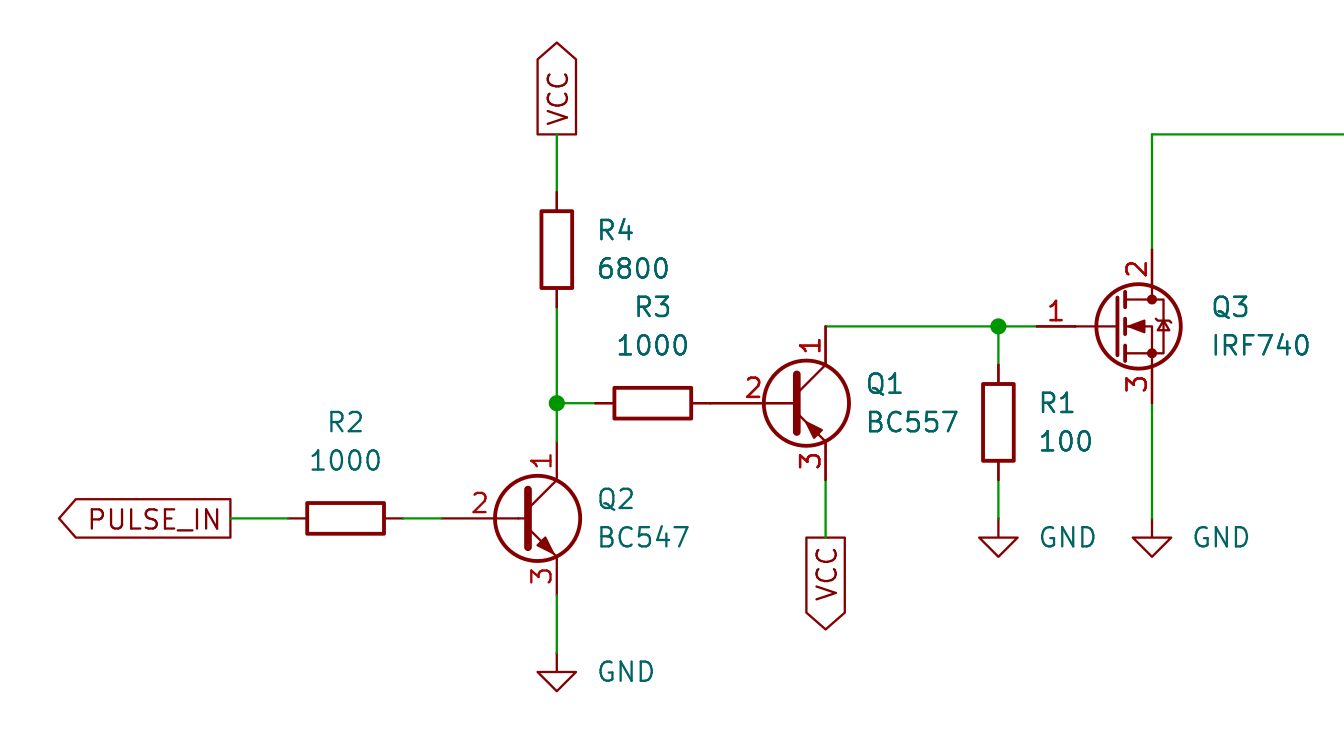
\includegraphics[width = 12cm]{img/budowa/sch/Sekcja_nadawcza.png}
    \caption{Schemat sekcji sterującej tranzystorem MOSFET przy użyciu sygnału \textit{PULSE\_IN}}
\end{figure}

Wygenerowany przez układ sterujący sekcją cyfrową sygnał prostokątny o napięciu $3,3V$ wzmacniany jest przez dwa tranzystory bipolarne $Q_2$, a następnie $Q_1$ połączone szeregowo pozwalające na uzyskanie wystarczającego napięcia do wysterowania tranzystora MOSFET IRF740 $Q_3$. Zastosowana konfiguracja tranzystorów bipolarnych pozwala na zminimalizowanie natężenia prądu wymaganego do wysterowania sekcji. Jest to szczególnie istotne biorąc pod uwagę fakt, że maksymalne natężenie oferowane przez zastosowany mikrokontroler wynosi $20mA$.
    
\begin{figure}[H]
    \centering
    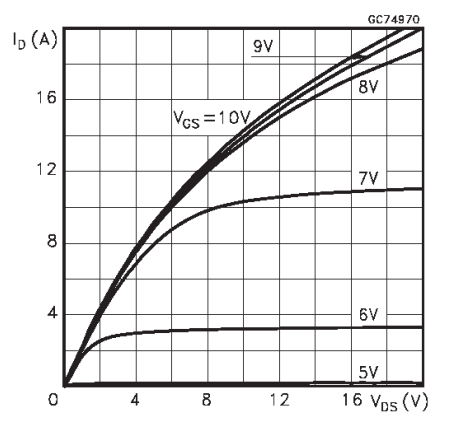
\includegraphics[width = 7.5cm, height = 7.5cm]{img/output_characteristics.png}
    \caption{Charakterystyka wyjściowa tranzystora IRF740}
    \hfill\small źródło: ST Microelectronics \cite{irf740} 
\end{figure}

\subsection{Pętla cewki}
\begin{figure}[H]
    \centering
    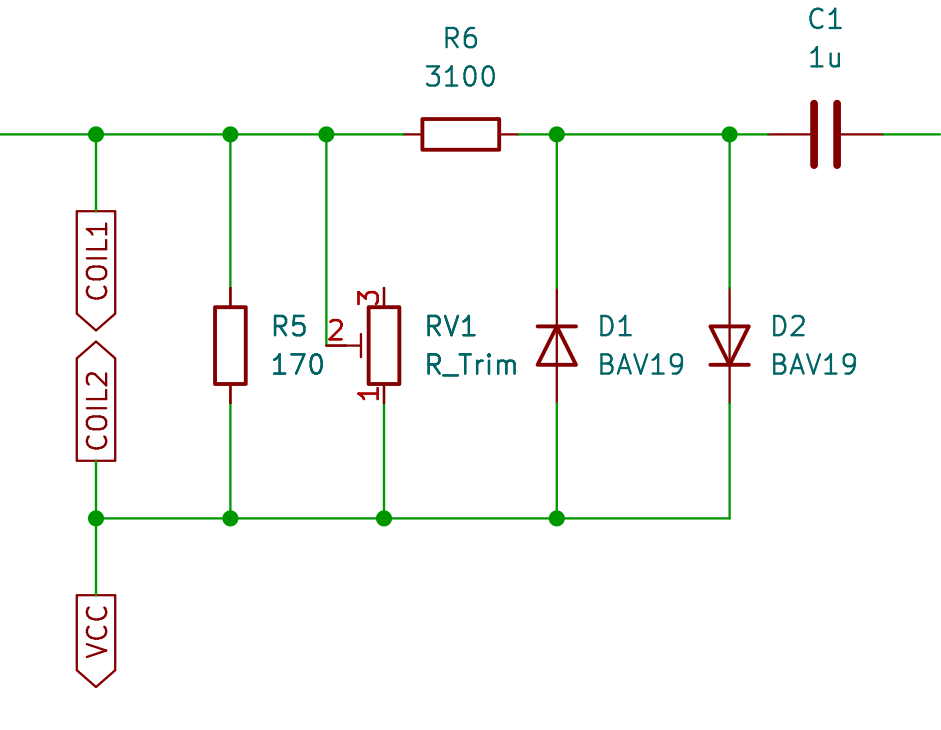
\includegraphics[width = 7.5cm]{img/budowa/sch/Pętla_cewki.png}
    \caption{Pętla rozładowująca cewkę}
\end{figure}

Tranzystor $Q_3$ zwiera sondę do masy powodując przepływ prądu przez cewkę podłączoną do \textit{COIL1} i \textit{COIL2}. Po otwarciu tranzystora $Q_3$ na cewce indukowane jest napięcie, którego górnym limitem jest przez napięcie breakdown $V_{brk}$ tranzystora wynoszące minimum $400V$ \cite{irf740}. W celu umożliwienia rozładowania napięcia w cewce zastosowano dwie szybkie diody typu \textit{BAV19} połączone równolegle odwrotnie do siebie pozwalające na przepływ prądu dla napięcia powyżej $0,7V$. Efekt jest opóźniony prez zastosowanie rezystora $R_6$. Dla końcowego etapu rozładowywania cewki, czyli kiedy napięcie jest poniżej progu przewodzenia diody rezystor $R5$ wraz z trymerem rezystorowym $RV1$ umożliwia przepływ prądu. Potencjometr zastosowany jest, aby łatwo dostroić tłumienie cewki w sposób inżynierski (zamiast wyznaczania wartości rezystora tłumiącego przy pomocy równania \ref{eq:pi_crit}). Pożądane jest krytyczne tłumienie odpowiedzi sondy pozwalające na najdokładniejsze pomiary zmian. Na rysunku \ref{eq:cewka_odp} narysowano porównanie odpowiedzi sondy nietłumionej oraz krytycznie tłumionej. Zademonstrowana odpowiedź jest mierzona za kondensatorem $C_1$.

\begin{figure}[H]
    \centering
    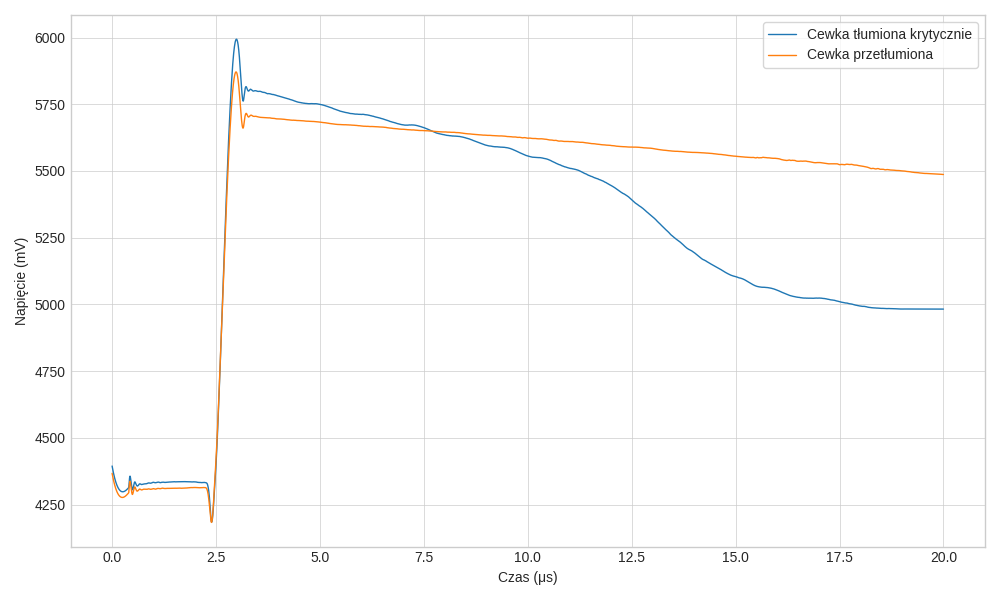
\includegraphics[width=0.8\textwidth]{img/budowa/coil_response.png}
    \caption{Wykres porównawczy odpowiedzi cewki}
    \label{eq:cewka_odp}
\end{figure}


\section{Sonda detekcyjna}
Sonda detekcyjna wykonana została z miedzianego przewodu o przekroju 0,4mm. Nawinięto 31 zwojów o średnicy 15cm.

Zgodnie z formułą Wheelera przedstawioną podczas przeglądu literatury indukcyjność cewki może zostać oszacowana w łatwy sposób. Jednostką miary w omawianym wzorze jest cal, więc wzór należy przekonwertować, aby móc z niego wygodnie skorzystać posiadając wymiary cewki w systemie metrycznym:
\begin{equation}
    L = \frac{0,8\cdot N^2 (\frac{a}{2,54})^2}{\frac{1}{2,54}\cdot(6a + 9b + 10c)}=\frac{0,315 \cdot N^2 a^2}{6a + 9b + 10c}
    \label{eq:cewka_id}
\end{equation}
gdzie a, b, c są wymiarami w centymetrach, N jest ilością zwojów w cewce.

\begin{equation}
    L=\frac{0,315 \cdot N^2 a^2}{6a + 9b + 10c}=\frac{0,315 \cdot 31^2 \cdot 7,5^2}{6 \cdot 7,5 + 9 \cdot 0,5 + 10 \cdot 0,5} \approx 312,4 \mu H
    \label{eq:cewka_obl}
\end{equation}


\section{Sekcja odbiorcza}


\begin{figure}[H]
    \begin{center}
    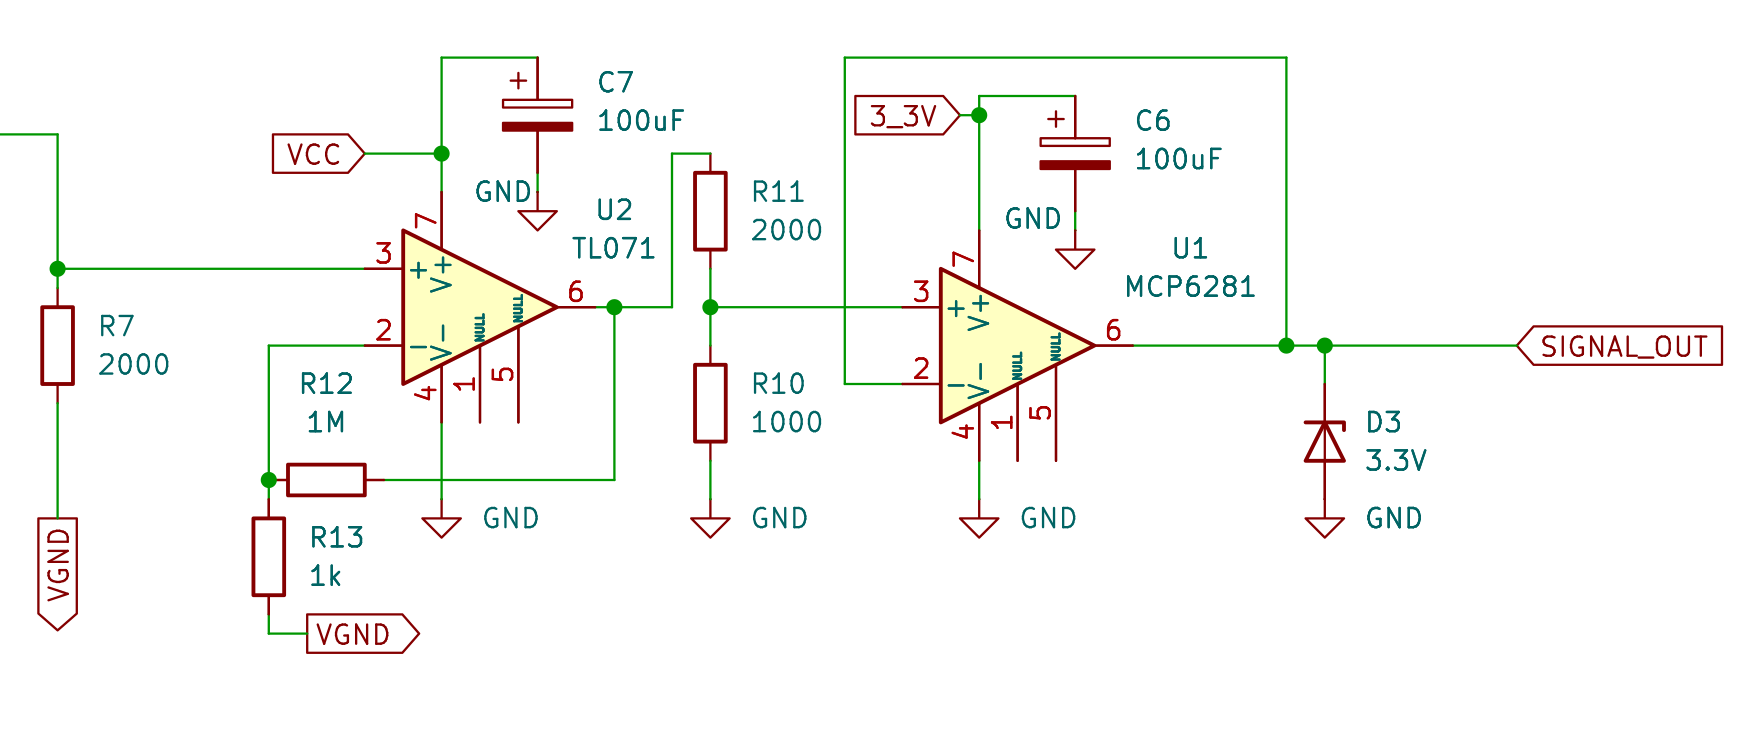
\includegraphics[width = 14cm]{img/budowa/sch/Sekcja_odbiorcza.png}
    \end{center}
    \caption{Schemat sekcji przetwarzającej sygnał odebrany przez sondę}
\end{figure}
Uzyskana odpowiedź z cewki po przejściu przez kondensator usuwający offset DC podciągana jest do napięcia $VGND$ za pomocą rezystora $R_7$. Następnie odpowiedź jest mnożona 1000-krotnie w celu uwydatnienia ostatniej części odpowiedzi sygnału najbardziej podatnej na działanie powstałego pola magnetycznego. Uzyskane napięcie może posiadać wartość zbliżoną do napięcia zasilania $V_{cc}$, dlatego w celu dostosowania go do poziomu pozwalającego obsłużyć go przez zastosowany w wykrywaczu MCU zastosowano dzielnik napięcia wykonujący mnożenie razy $0,33$. Tak wyznaczony sygnał nie jest wystarczająco silny, dlatego przechodzi on przez kopiujący wzmacniacz $U_1$. Warto zaznaczyć, że wzmacniacz MCP6281 jest typu rail-to-rail, pozwalający na operowanie na sygnałach bliskich napięciom zasilania $V_+$, jak i $V_-$ wzmacniacza \cite{mcp6281_ds}. Poprzednie sekcje nie wymagały tej specjalnej właściwości. Tak przygotowany sygnał jest gotowy do analizy przez mikrokontroler. Dla dodatkowego bezpieczeństwa zastosowano diodę zenera $3,3V$ gwarantującą, że \textit{SIGNAL\_OUT} należy do zakresu napięć obsługiwanego przez sekcję cyfrową.


\subsection{Wirtualna masa}
\begin{figure}[H]
    \begin{center}
    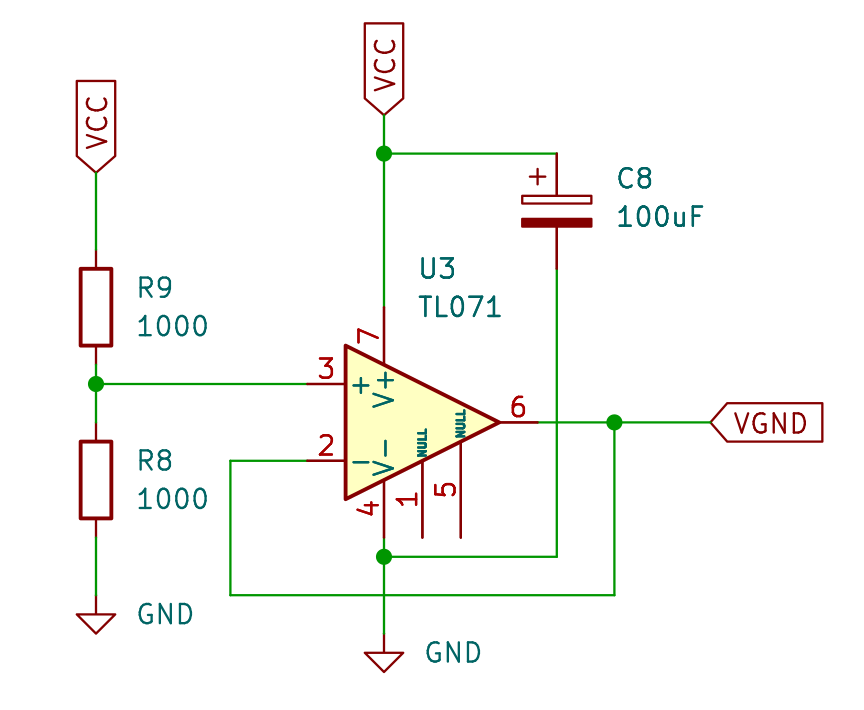
\includegraphics[width = 7.5cm]{img/budowa/sch/Wirtualna_masa.png}
    \end{center}
    \caption{Konfiguracja wzmacniacza operacyjnego generującego napięcie $VGND$}
\end{figure}

W celu uzyskania pełnej odpowiedzi cewki zastosowana jest sztuczna masa wynosząca połowę napięcia zasilania. Dzięki niej wzmacniacze operacyjne w sekcji wzmocnienia odpowiedzi mogą wzmocnić odpowiedź pracując wyłącznie z dodatnim napięciem, co omija konieczność generowania ujemnego napięcia upraszczając finalny schemat wykrywacza metalu. Wykonana jest za pomocą dzielnika napięcia wykonującego działanie

\begin{equation}
    U_{VGND}=Vcc\cdot\frac{R9}{R8+R9}=Vcc\cdot\frac{1}{2}  
    \label{eq:vgnd}
\end{equation}
którego wynikowe napięcie przechodzi przez wzmacniacz operacyjny $U3$ kopiujący napięcie wejściowe wzmacniając sygnał, jednocześnie odciążając zastosowane w dzielniku rezystory.



\section{Sekcja cyfrowa}

\begin{figure}[H]
    \begin{center}
        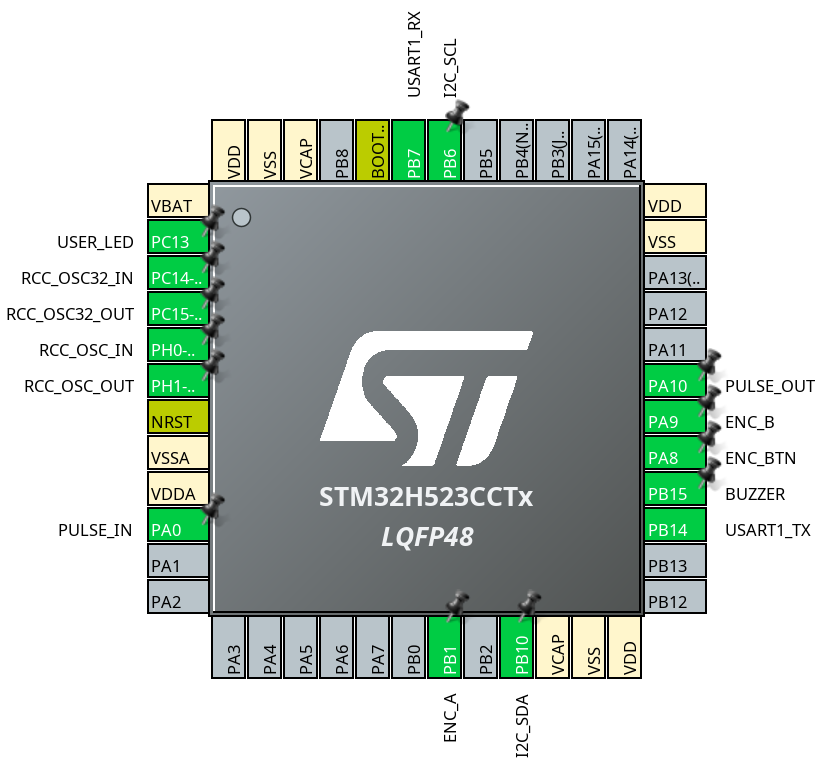
\includegraphics[width=7.5cm]{img/budowa/cube_mx.png}
    \end{center}
    \caption{Cyfrowe przedstawienie układu STM32H523CE wraz z użytymi portami}\label{fig:stm32}
\end{figure}


Część cyfrowa wykrywacza metalu oparta jest o moduł STM32H523CECoreBoard \cite{WeActStudio_STM32H523CoreBoard} zawierający układ \textbf{STM32H523CE}. Ten produkowany przez ST Microelectronics mikrokontroler posiada jeden 32-bitowy rdzeń oparty na architekturze ARM\textregistered{} Cortex-M33\textregistered{} \cite{st_stm32h5_web} \cite{st_stm32h533_ds} o maksymalnym taktowaniu 250Mhz oraz m.in wykorzystane w projekcie układy peryferyjne:

\subsection{Liczniki sprzętowe}
\label{subsec:timery}
Wykorzystywane są dwa 16-bitowe liczniki sprzętowe napędzane za pomocą zegara \textit{APB2} skonfigurowanego na taktowanie z częstotliwością $F_{timer}=250Mhz$.

Konfiguracja oraz interakcja z licznikami w rodzinie układów STM32 odbywa się za pomocą rejestrów:
\begin{itemize}
    \item PSC (Dzielnik, ang. \textit{Prescaler}) - dzieli częstotliwość wejściową $F_{timer}$
    \item ARR (Rejestr Automatycznego Przeładowania, ang. \textit{Auto Reload Register}) - określa długość całego cyklu, po przeładowaniu następuje reset licznika
    \item CCR (Rejestr Przechwytywania i Przeładowania, ang. \textit{Capture/Compare Register}) - w trybie PWM określa moment przełączenia sygnału
    \item CNT (Licznik, ang. \textit{Counter}) - przechowuje aktualną liczbę tyknięć licznika
\end{itemize}

Częstotliwość przepełnienia licznika sprzętowego można wyznaczyć za pomocą poniższego równania: 

\begin{equation}
    F_{output}=\frac{F_{timer}}{(PSC+1)(ARR+1)}
    \label{eq:timer_f}
\end{equation}


Licznik \textit{TIM1} pełni funkcję generatora sygnału \textit{PULSE\_OUT} za pomocą trybu sprzętowego trybu modulacji szerokości impulsów.
Pozwala on na konfigurację częstotliwości oraz wypełnienia sygnału przez mikrokontroler. Jeżeli wartość rejestru \textit{CNT} jest mniejsza od \textit{CCR}, wystawiany jest sygnał +3,3V na pin 1 (PULSE\_OUT) układu, powodując otwarcie tranzystora MOSFET. Następnie w pożądanym momencie sygnał wyjściowy jest wygaszony, co pozwala na dynamiczną konfigurację długości impulsu wysyłanego do cewki.

Drugi licznik \textit{TIM12} wykorzystany jest do generowania sygnału PWM o wypełnieniu 50\% i dynamicznie wyznaczanej częstotliwości do brzęczyka wskazującego o wykryciu anomalii w przetworzonym sygnale \textit{SIGNAL\_OUT}.
Dynamiczna rekonfiguracja rejestrów licznika pozwala na uzyskanie tonu o zadanej częstotliwości. 
Wzór na wartość rejestru ARR można wyznaczyć przekształcając wzór \ref{eq:timer_f}:

\begin{equation}
    ARR = \frac{F_{timer}}{(PSC+1) \cdot f_{target}} - 1
    \label{eq:buzzer_arr}
\end{equation}

W celu uzyskania wypełnienia 50\% należy ustawić rejestr \textit{CCR} na połowę wartości rejestru \textit{ARR}:

\begin{equation}
    CCR = \frac{ARR}{2}
    \label{eq:buzzer_ccr}
\end{equation}

\subsection{Konwerter cyfrowo-analogowy}

ADC napędzany jest sygnałem zegarowym \textit{HCLK} o częstotliwości $F_{ADC}=250Mhz$, z preskalerem o wartości $4$, co daje końcową częstotliwość podukładu wynoszącą $62,5Mhz$.
Maksymalna rozdzielczość pomiaru wynosi 12 bitów, co daje dokładność na poziomie $0,8 mV$.

\begin{equation}
R= \frac{Vref}{2^N - 1} =\frac{3,3V}{4095}\approx 0,8mV
\end{equation}

gdzie $V_{ref}$  to napięcie referencyjne (tutaj $V_{in}=3,3V$), $N$ = liczba bitów

W celu osiągnięcia jak największego zasięgu wykrywacza wymagana jest jednocześnie jak największa dokładność układu ADC oraz jego szybkość działania. Dla trybu 12-bitowego każdy pomiar zajmuje $C_{sample}=15$ cykli zegarowych dających teorytyczny limit przy ustalonym wcześniej taktowaniu zegara ADC wynoszący $4,16 MSPS$ (milionów próbek na sekundę, ang. \textit{Mega Sample Per Second}), co daje jedną próbkę napięcia co $~0,24\mu s$.

\begin{equation}
    SPS = \frac{F_{ADC}}{C_{sample}}=\frac{62,5\cdot10^6}{15}\approx{4,16\cdot10^6}\frac{S}{s}
\end{equation}

Dla maksymalnego odciążenia mikrokontrolera wykorzystany został tryb DMA (bezpośredni dostęp do pamięci, ang. \textit{Direct Memory Access}) z wyłączonym generowaniem przerwań sprzętowych. Każda nowa próbka napięcia wykonana przez konwerter analogowo-cyfrowy zapisywana jest przez układ peryferyjny GPDMA1 do cyklicznego buforu znajdującym się pamięci SRAM wskazanym podczas konfiguracji bez dodatkowego udziału rdzenia Cortex-M33.

\begin{figure}[H]
    \begin{center}
        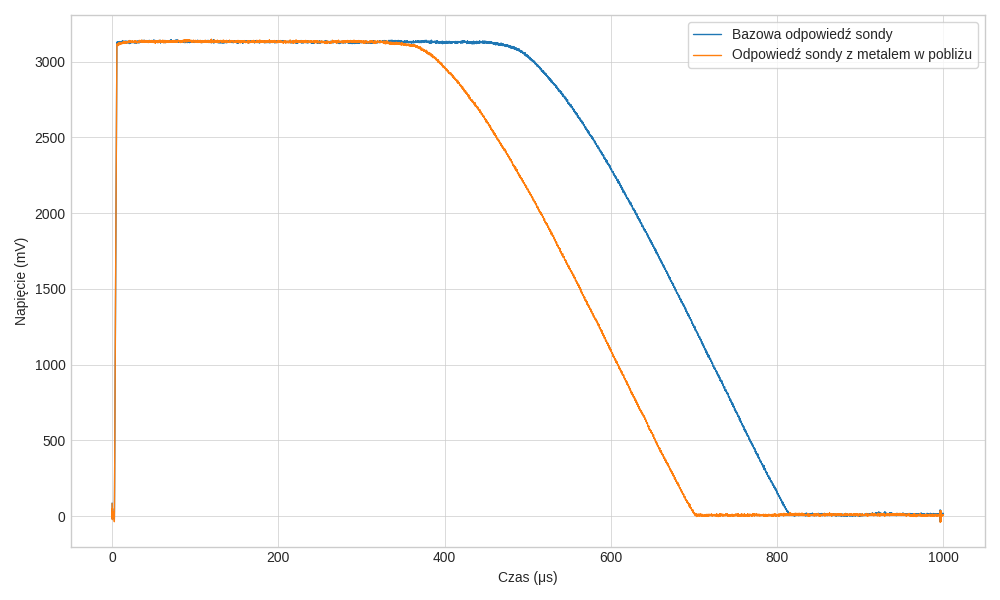
\includegraphics[width=0.95\textwidth]{img/budowa/pulse_out.png}
    \end{center}
    \caption{Wykres odpowiedzi sondy \textit{PULSE\_OUT}}\label{fig:pulse_out}
\end{figure}

W celu dokładnego wyznaczenia trwania nasyconej odpowiedzi sondy wykorzystywany jest wbudowany w ADC sprzętowy komparator okienkowy (Analog Watchdog, AWD). To peryferium konwertera analogowo-cyfrowego pozwala na wyznaczenie zakresu wartości próbek, którego opuszczenie wywoła przerwanie mikrokontrolera. W prototypie moduł ten skonfigurowany jest na wykrywanie momentu przekroczenia przez sygnał wartości dolnej granicy wynoszącej 3000. Górna granica okna wynosi 4095, czyli maksymalną wartość próbki przy rozdzielczości 12-bitów, efektywnie eliminując możliwość wywołania przerwania.


Algorytm napędzający prototyp wykrywacza metali wykorzystuje komparator okienkowy w celu wykrywania anomalii czasu trwania odpowiedzi sondy.
Jak można zauważyć na wykresie \ref{fig:pulse_out}, podczas przybliżenia metalowego obiektu zmienia się charakterystyka sygnału \textit{SIGNAL\_OUT}.
Wykorzystanie sprzętowego rozwiązania pozwala na dokładne wyznaczenie momentu przekroczenia granicy 2,01V ($\frac{2500}{4095}\cdot 3,3V$). Kod przerwania wywołanego przez AWD zapisuje w pamięci mikrokontrolera aktualną wartość licznika \textit{TIM1}, co pozwala dokładnie odtworzyć względny czas wywołania przerwania po wyłączeniu sygnału \textit{PULSE\_OUT}. Przechwycona wartość mnożona jest przez czas pomiędzy inkrementacją licznika.


\section{Płytka drukowana}
Płytka drukowana (PCB, ang. \textit{Printed Circuit Board}) prototypu została zaprojektowana w otwartoźródłowym programie typu CAD (projektowanie wspomagane komputerowo, ang. \textit{Computer Aided Design}) KiCad\cite{kicad}.
Finalny produkt został wykonany z wykorzystaniem laminatu dwustronnego o wymiarach $80mm$ x $101mm$.
W celu minimalizacji zakłóceń elektromagnetycznych, wolne przestrzenie na obu warstwach PCB zostały wypełnione wylewką miedzi (ang. \textit{copper pour}) podłączoną do potencjału masy.

\begin{figure}[H]
\centering
  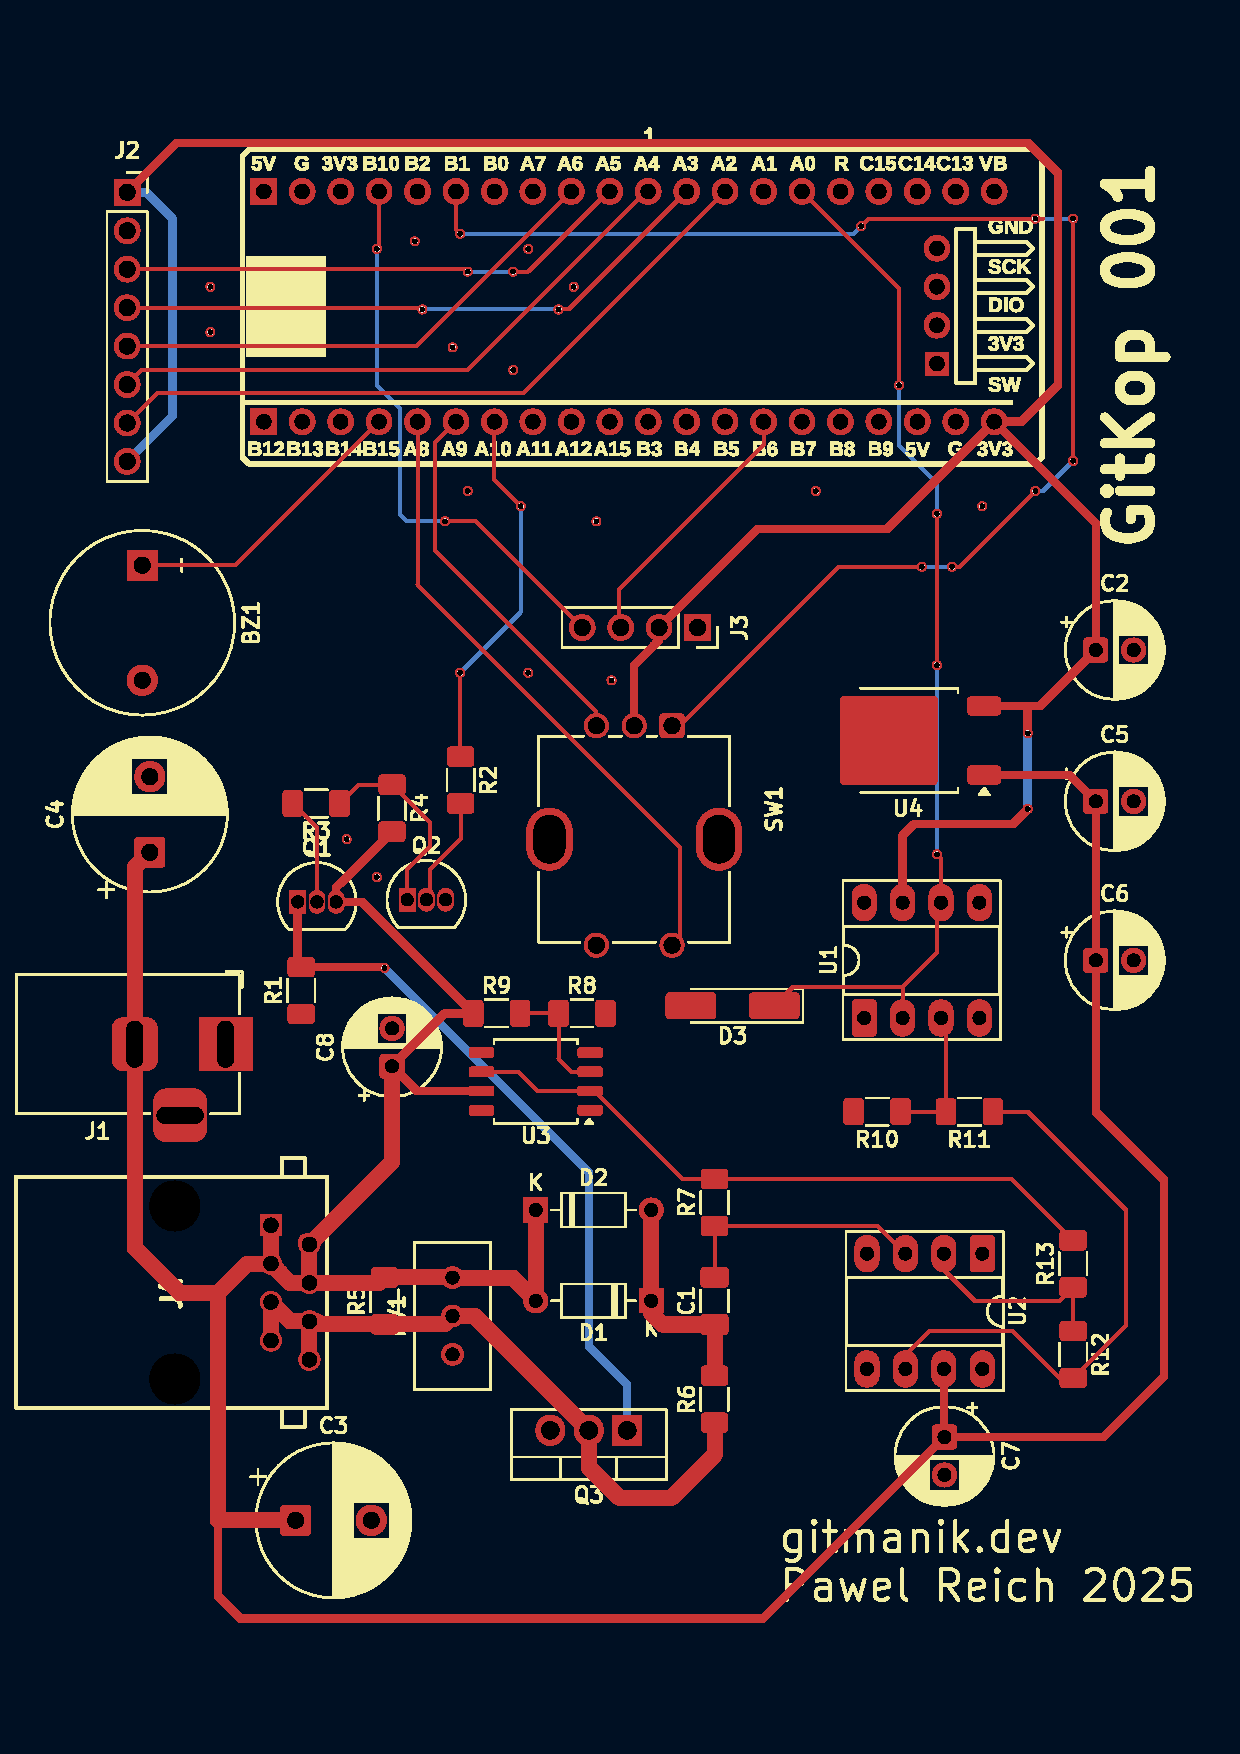
\includegraphics[width=0.5\textwidth]{./pcb.pdf}
  \caption{Schemat projektu PCB (z pominiętą płaszczyzną masy)}
\end{figure}

\begin{figure}
\centering
  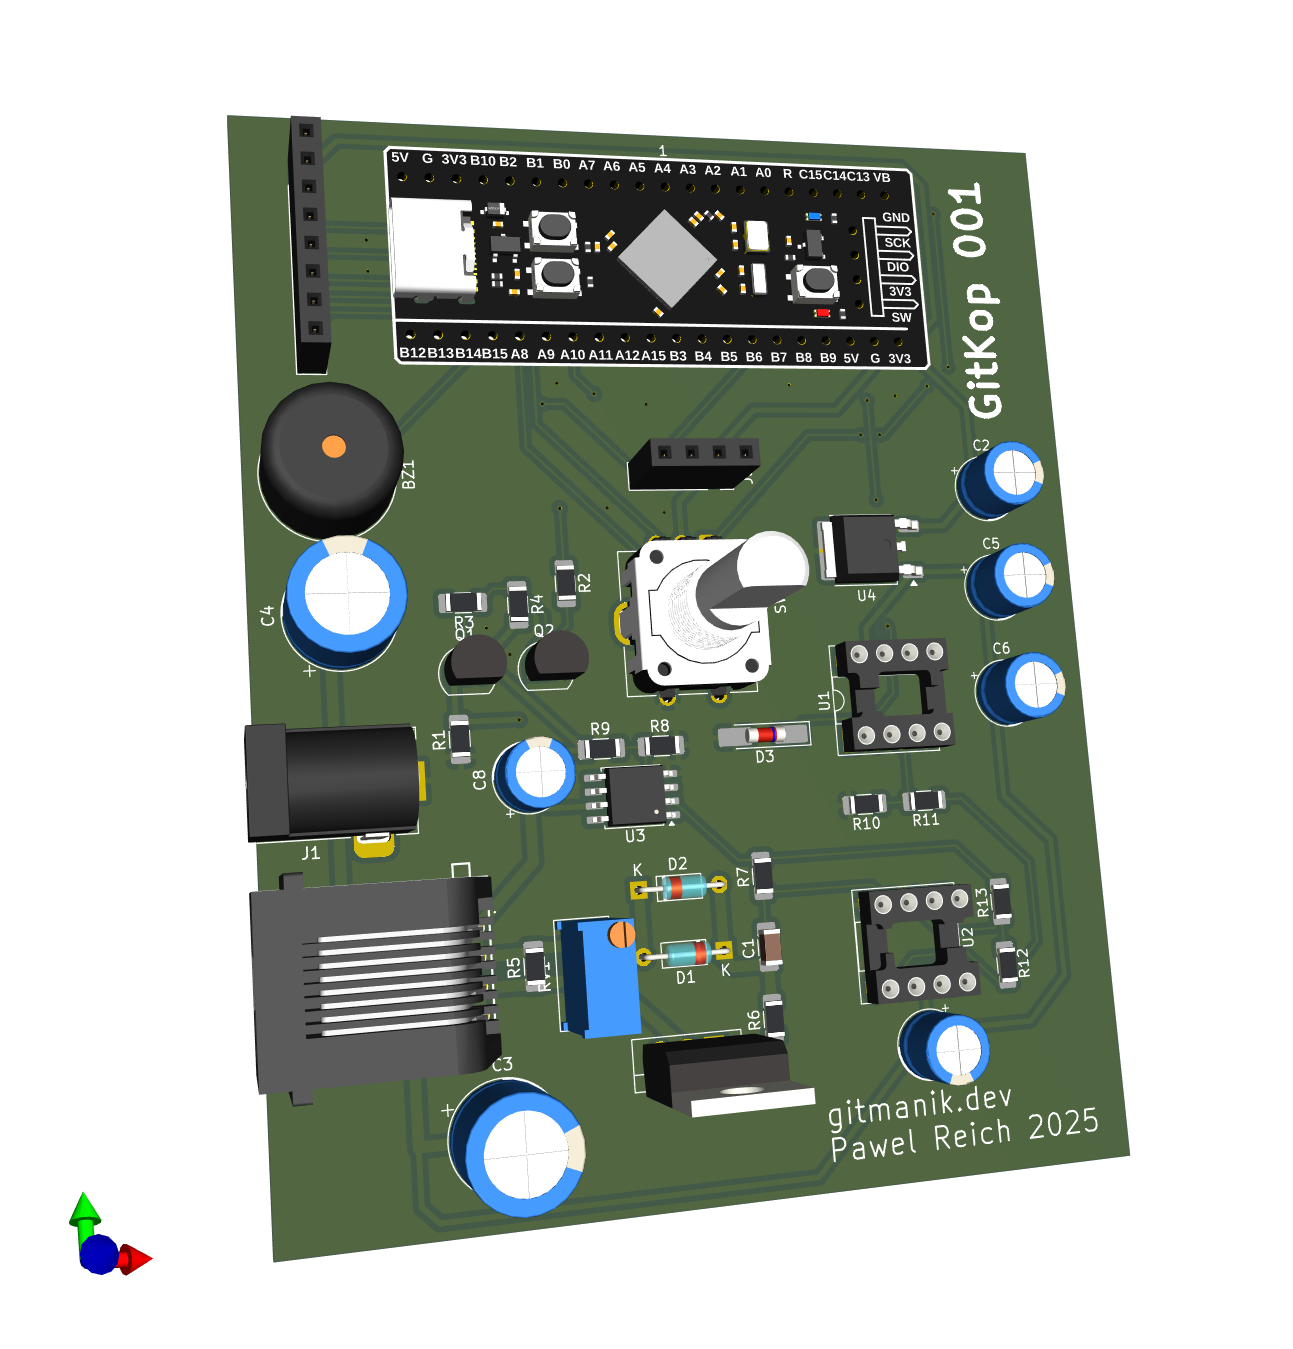
\includegraphics[width=0.7\textwidth]{./img/pcb_3drender.png}
  \caption{Trójwymiarowe komputerowe przedstawienie projektu PCB}
\end{figure}

\section{Obudowa}
Obudowa wykrywacza metalu została wykonana w technologii druku 3D z wykorzystaniem plastiku PET-G gwarantującym większą wytrzymałość mechaniczną w porównaniu
do alternatyw.
Głównym założeniem projektowym było stworzenie kompaktowej konstrukcji. Wymiary zewnętrzne obudowy wynoszą odpowiednio $85mm$ x $126mm$ x $28mm$.
Projekt posiada dedykowane otwory na port sondy RJ45 oraz gniazdo zasilające DC.
Całość zamykana jest poprzez cztery śruby M3, wkręcane we wkładki metalowe montowane na gorąco.
Obudowa PCB została zaprojektowana w oprogramowaniu CAD 3D Autodesk Fusion.

\begin{figure}
    \begin{center}
        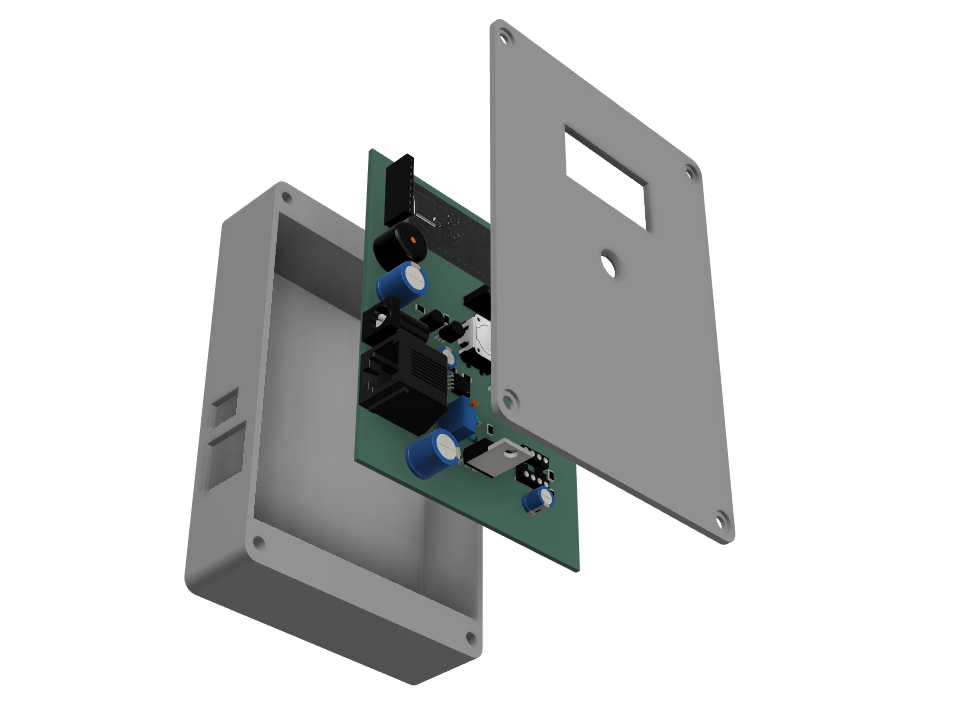
\includegraphics[width=\textwidth]{img/pudlo otwarte.png}
    \end{center}
    \caption{Trójwymiarowe przedstawienie PCB zamkniętego w zaprojektowanej obudowie}
\end{figure}


\chapter{Testy i analiza skuteczności}

Podczas analizy pracy oraz wykonywania pomiarów prototyp był zasilany napięciem $10V$ pochodzącym z liniowego zasilacza laboratoryjnego zapewniającego stabilne zasilanie.

Podczas testów urządzenie generowało sygnał \textit{PULSE\_OUT} o częstotliwości 1kHz i wypełnieniu 1,5\%

\section{Oprogramowanie zarządzające}

W celu zwizualizowania, zarządzania urządzeniem oraz wykreślenia danych testowych generowanych w czasie rzeczywistym przezwykrywacz metalu powstał program zarządzający.
Napisany w języku Python, łączy się z urządzeniem za pomocą peryferium \textit{USART1} (Uniwersalny Synchroniczny Asynchroniczny Nadajnik-Odbiornik, ng. \textit{Universal Synchronous Asynchronous Receiver Transmitter}) wbudowanego w mikrokontroler.
Połączenie z komputerem następuje dzięki urządzeniu ST-Link oferującemu, oprócz interfejsu SWD (Szeregowy interfejs debugowania, ang. \textit{Serial Wire Debug}), konwerter komunikacji szeregowej TTL (logika tranzystor-tranzystor, ang. \textit{Transistor-Transistor Logic}). Dzięki zastosowaniu języka Python, program pozwala na szybką iterację, przetwarzanie oraz prezentację danych generowanych przez wykrywacz. 

\begin{figure}[H]
    \centering
    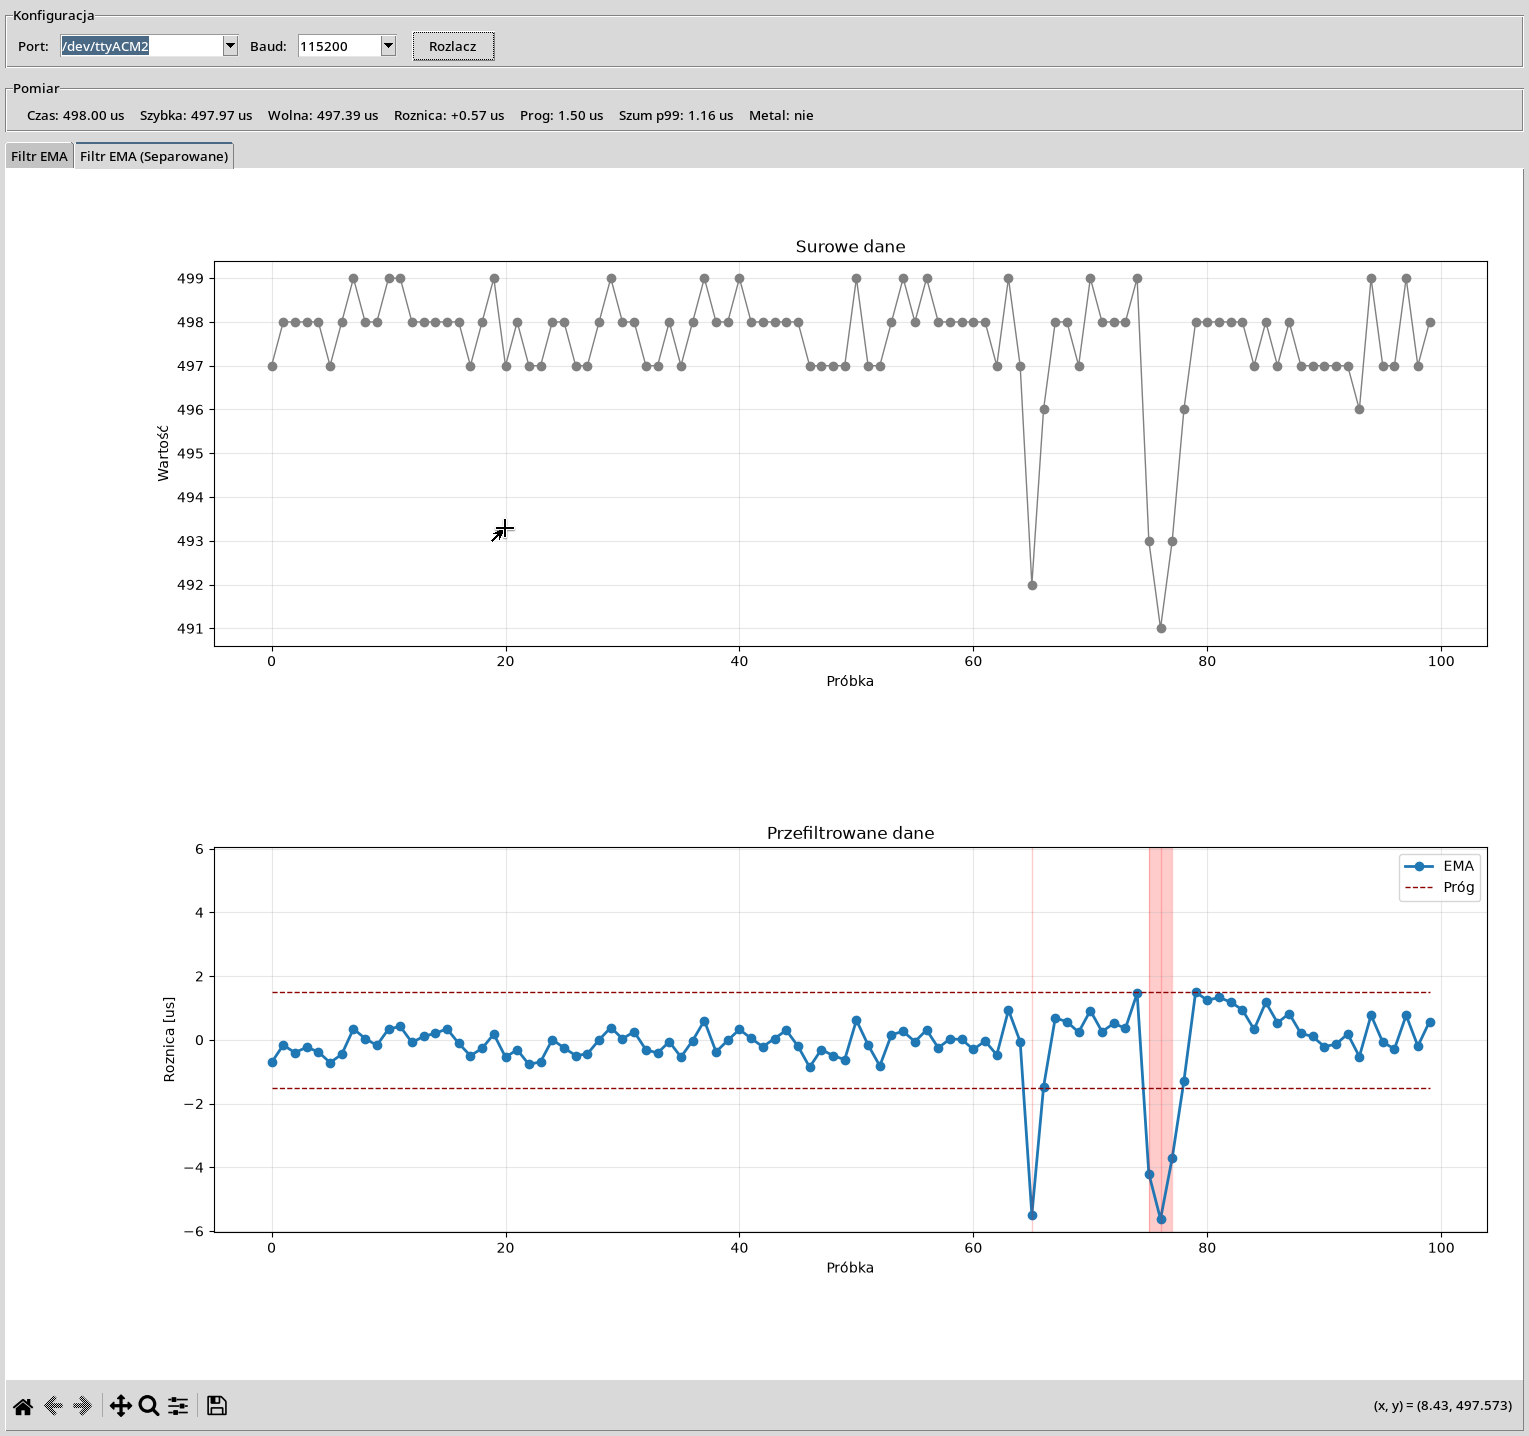
\includegraphics[width=0.7\textwidth]{img/soft.png}
    \caption{Zrzut ekranu oprogramowania zarządzającego}\label{fig:test_program}
\end{figure}


\section{Algorytm wyznaczania danych wejściowych}

\begin{figure}
    \centering
    \begin{tikzpicture}[node distance=1cm, auto]

        \node (start) [startstop] {Start};
        \node (fast) [process, below=of start] {Wyznacz nową wartość \\szybkiego filtru};
        \node (slow) [process, below=of fast] {Wyznacz nową wartość \\wolnego filtru};
        \node (dec) [decision, below=of slow] {Czy\\$S_f - S_s > T_h$ ?};
        \node (change) [process, below=of dec, node distance=2.5cm] {Wyznacz zmianę\\napięcia w\\czasie};
        \node (signal) [process, below=of change] {Uruchom\\sygnalizację\\akustyczną};
        \node (end) [startstop, below=of signal] {Koniec};

        \draw [arrow] (start) -- (fast);
        \draw [arrow] (fast) -- (slow);
        \draw [arrow] (slow) -- (dec);
        
        \draw [arrow] (dec) -- node[anchor=east] {Tak} (change);
        \draw [arrow] (change) -- (signal);
        \draw [arrow] (signal) -- (end);
        
        \draw [arrow] (dec.east) -- ++(2.5,0) node[midway, above] {Nie} |- (end.east);

    \end{tikzpicture}
    \caption{Schemat blokowy działania algorytmu}\label{fig:diagram}
\end{figure}

\subsection{Filtracja sygnału pomiarowego i detekcja obiektu}

Ze względu na charakter wzmocnionego sygnału wyjściowego z sekcji odbiorczej, który obarczony jest znacznym szumem o charakterze stochastycznym, a także szumom wynikającym z przetwornika analogowo-cyfrowego konieczne było zastosowanie odpowiednich metod cyfrowego przetwarzania sygnałów. Wstępna analiza widmowa z wykorzystaniem Szybkiej Transformaty Fouriera (FFT) wykazała, że zakłócenia mają charakter szerokopasmowy (szum biały), co uniemożliwia skuteczne odfiltrowanie ich poprzez proste wycięcie konkretnych częstotliwości bez utraty istotnych informacji o zmianach sygnału użytecznego. W związku z tym, do kondycjonowania sygnału wybrano filtr dolnoprzepustowy w dziedzinie czasu.

\subsection{Charakterystyka filtru EMA}

Wykładnicza średnia krocząca  (ang. \textit{Exponential Moving Average}, EMA) jest filtrem o nieskończonej odpowiedzi impulsowej (IIR), który przypisuje wagi do danych historycznych w sposób malejący wykładniczo. Jest to rozwiązanie szczególnie korzystne w systemach wbudowanych o ograniczonych zasobach obliczeniowych, ponieważ nie wymaga buforowania dużej liczby próbek, a jedynie przechowywania poprzedniej wartości przefiltrowanej.

Równanie rekurencyjne filtru EMA opisuje wzór:

\begin{equation}
    S_t = \alpha \cdot Y_t + (1 - \alpha) \cdot S_{t-1}
    \label{eq:ema}
\end{equation}

gdzie $S_t$ - aktualna wartość przefiltrowana, $Y_t$ - aktualna surowa wartość, $S_{t-1}$ - poprzednia wartość przefiltrowana, $\alpha$ - współczynnik wygładzania z przedziału $(0, 1)$.

Współczynnik $\alpha$ decyduje o stałej czasowej filtru. Niska wartość $\alpha$ skutkuje silnym tłumieniem szumu, ale wprowadza większe opóźnienie w detekcji szybkich zmian sygnału. Wysoka wartość $\alpha$ zapewnia szybszą reakcję układu, lecz słabiej eliminuje zakłócenia o wysokiej częstotliwości.

\subsection{Algorytm detekcji różnicowej}

W celu eliminacji efektu pływania zera w algorytmie zastosowano dodatkowa średnią z filtrem EMA o niskiej wartości $\alpha$, reprezentującą tło.

Warunek detekcji metalu opiera się na analizie różnicy między tymi dwoma sygnałami, co przedstawia nierówność (\ref{eq:trigger}):

\begin{equation}
    Diff=S_{fast} - S_{slow} > T_{h}
    \label{eq:trigger}
\end{equation}

gdzie $Diff$ to wyznaczona różnica, $S_{fast}$ to aktualna wartość szybkiego filtra EMA, $S_{slow}$ to aktualna wartość wolnego filtra EMA, $T_{h}$ to próg detekcji.

Zaletą zastosowania dwóch średnich jest automatyczna kalibracja układu. W stanie spoczynku różnica $Diff$ oscyluje wokół zera, niezależnie od bezwzględnej wartości odpowiedzi sygnału z cewki. W momencie pojawienia się obiektu metalowego, $S_{fast}$ narasta znacznie szybciej niż $S_{slow}$, powodując przekroczenie progu $T_{h}$.


\subsection{Nachylenie odpowiedzi}

Podczas wykonywania algorytmu wykrywania kopiowany jest segment bufora cyklicznego uzupełnianego przez DMA do bufora $x$ zawierajego ostatnie $N=42$ próbek. Dokonywany jest proces analizy nachylenia sygnału.

\begin{equation}
    N = \frac{T}{SPS}=\frac{10\mu s}{4,16\cdot10^6 \frac{S}{s}} \approx{42}
\end{equation}

Nachylenie sygnału wyznaczane jest za pomocą uproszczonego uśrednienia zmiany napięcia:
\begin{equation}
    Delta = \frac{x[N] - x[0]}{N}
    \label{eq:nachyl}
\end{equation}

\section{Test działania wykrywacza}

Podczas pracy wykrywacza pobierany prąd zawarty był w zakresie $(70mA - 80mA)$, przy przyjętym wcześniej napięciu zasilania $12V$ daje to stałe obciążenie około $0,9W$.

Urządzenie poprawnie wyznacza czas trwania odpowiedzi sondy, wraz z filtracją szumów. Na rysunku \ref{fig:filtry_wewnetrzne} wykreślono surowe, pomierzone dane próbek wraz ze stanami filtrów EMA oraz końcowym, wynikowym sygnałem
będący podstawą do podjęcia decyzji o stwierdzonej anomalii sygnału. Na wykresie \ref{fig:filtry_wykryte} zauważyć można zmianę wartości spowodowaną obecnością obiektu badanego w pobliżu.


\begin{figure}
    \centering
    \includesvg[width=\textwidth]{img/testy/filtry.svg}
    \caption{Wykres wewnętrznych stanów wykrywacza}\label{fig:filtry_wewnetrzne}
\end{figure}

\begin{figure}
    \centering
    \includesvg[width=\textwidth]{img/testy/filtry_wykryte.svg}
    \caption{Wykres wewnętrznych stanów wykrywacza ze zbliżonym tymczasowo obiektem}\label{fig:filtry_wykryte}
\end{figure}



\section{Analiza skuteczności działania urządzenia} 

Analiza została przeprowadzona z wykorzystaniem metalowego obiektu badanego (widocznego na rysunku \ref{fig:obiekt_badany}) oddalonego od sondy wykrywacza na 15 cm.


\begin{figure}
    \centering
    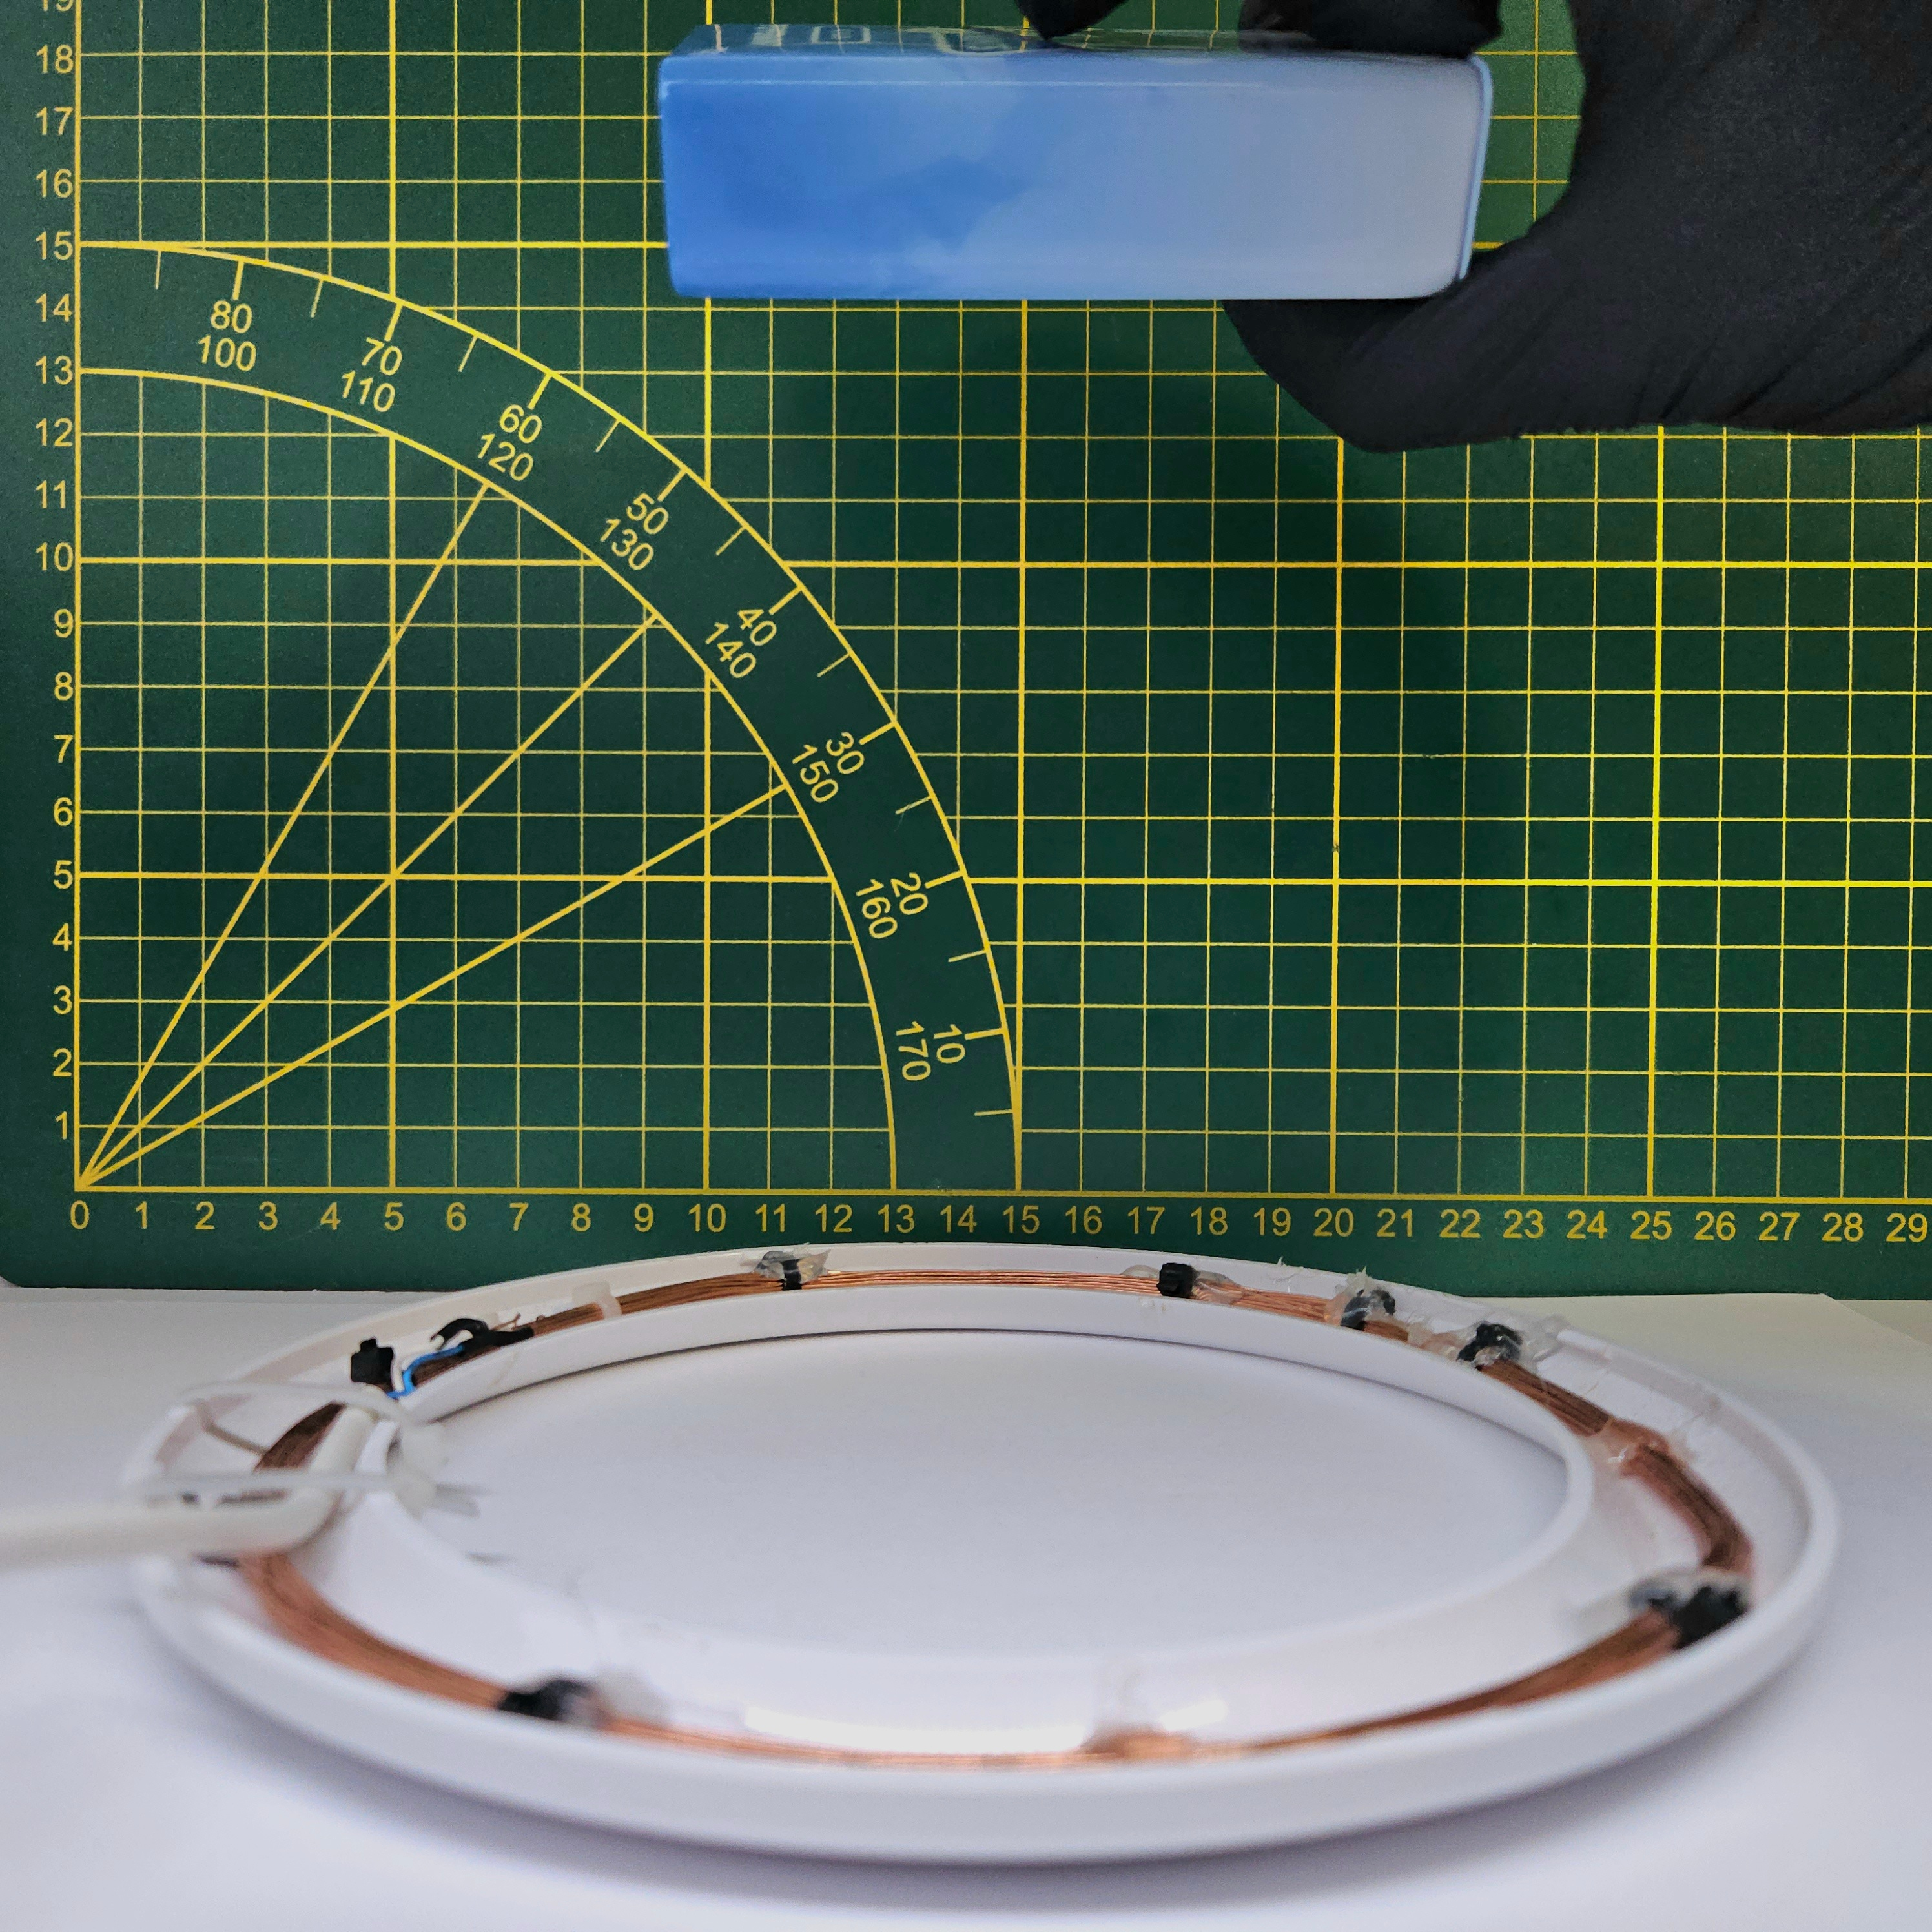
\includegraphics[width=0.7\textwidth]{img/testy/obiekt.jpg}
    \caption{Obiekt zastosowany podczas analizy skuteczności wykrywacza metali}
    \label{fig:obiekt_badany}
\end{figure}

Jak widać na wykresie \ref{fig:test_obiekt} urządzenie poprawnie reaguje na obecność obiektu.
Fluktuacja stanu przekracza próg anomalii generując sygnał akustyczny (zaznaczony na wykresie).

\begin{figure}
    \centering
    \includesvg[width=\textwidth]{img/testy/surowe_wykryte.svg}
    \caption{Wykres stanu wykrywacza w czasie, z zakolorowanymi segmentami ze stwierdzoną anomalią}
    \label{fig:test_obiekt}
\end{figure}



\printbibliography

\begin{appendices}
    \appendix
    \include{pcb}
    \chapter{Schemat gotowego wykrywacza metalu}
    \begin{figure}[H]
        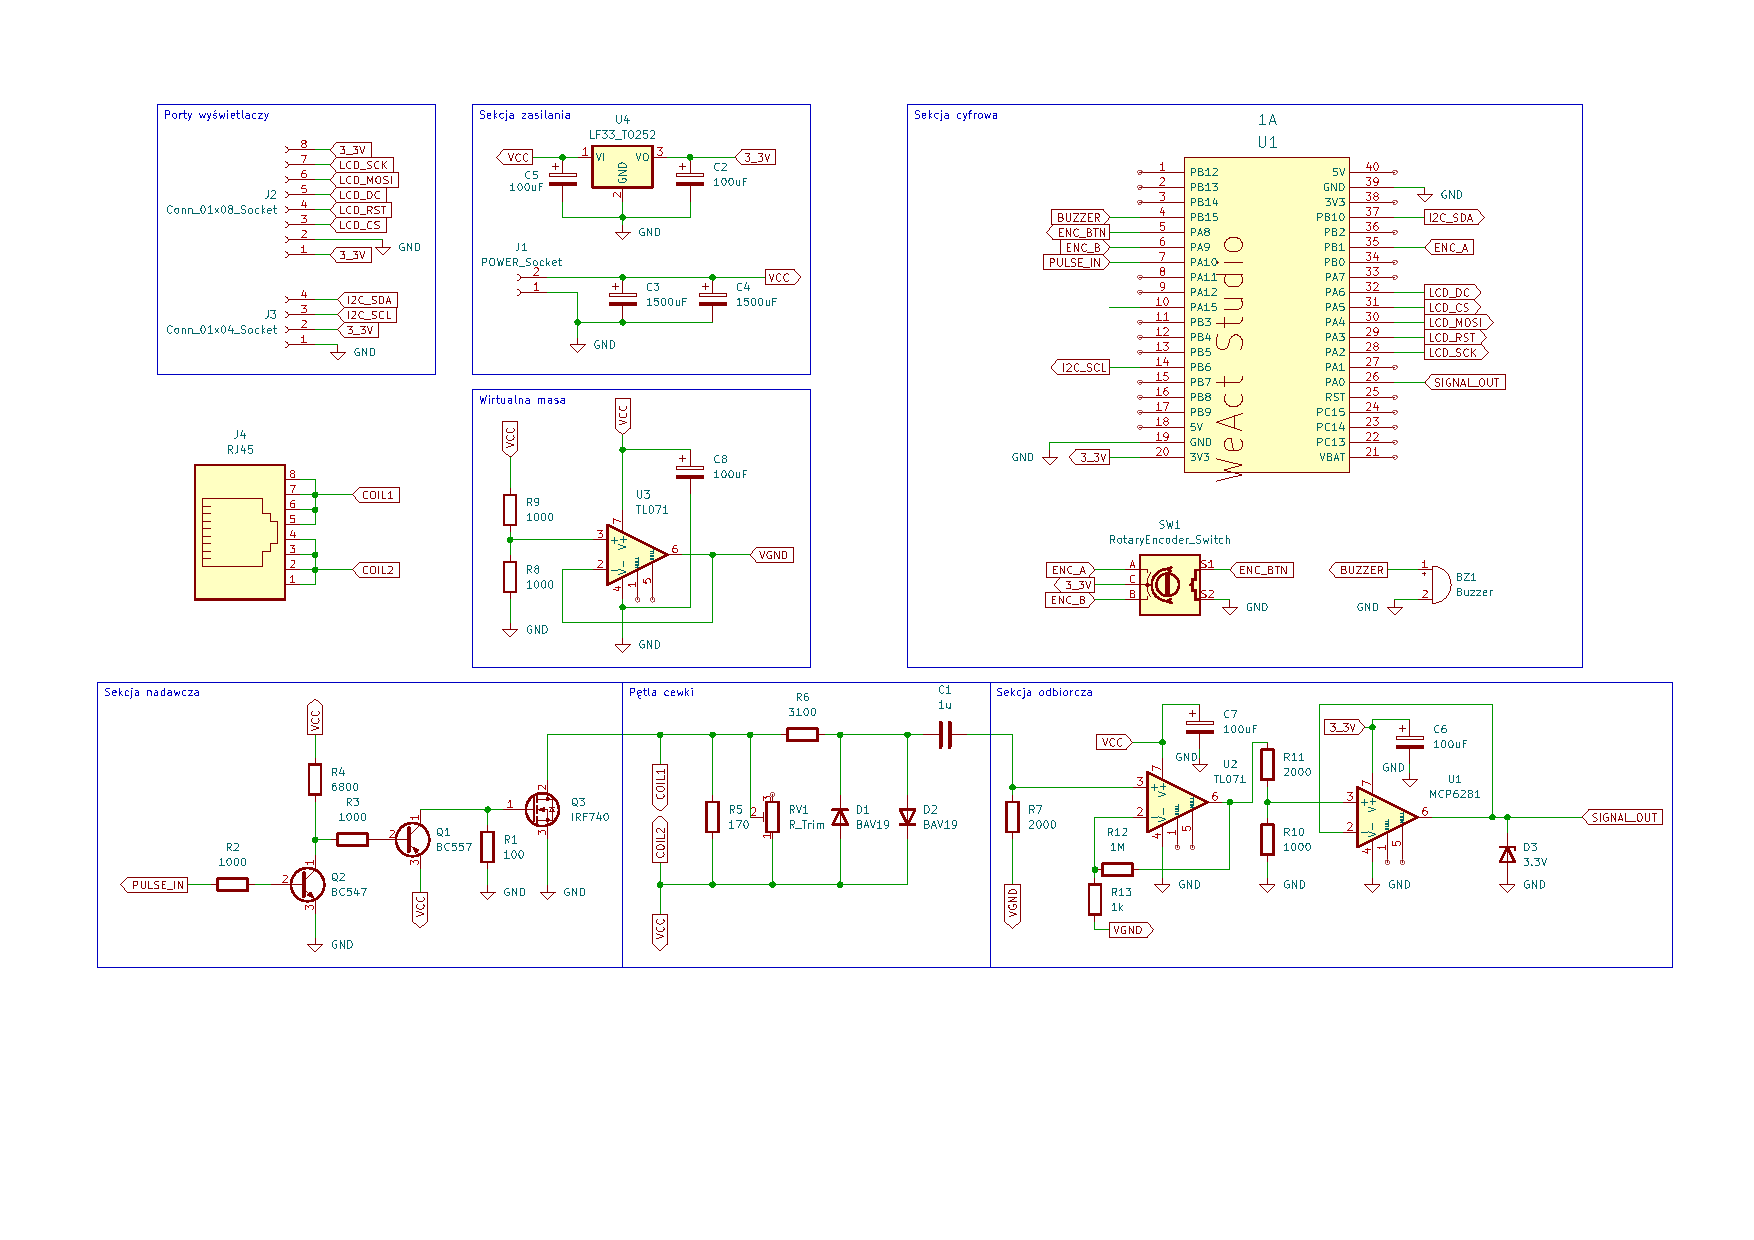
\includegraphics[angle=90, width=\textwidth]{Schematic.pdf}
    \end{figure}
\end{appendices}

\end{document}
